\chapter{Sistema Mecânico}

O robô utilizado no projeto é o mesmo robô construído durante o projeto \textbf{Robô Explorador de Labirintos 2D} \cite{RoboExplorador} desta mesma disciplina.

No projeto original o robô era utilizado para explorar e solucionar labirintos em duas dimensões feitos através de trilhas pretas em um chão branco, utilizado emissores e sensores de luz infravermelha para identificar a pista. 

Todo o projeto mecânico foi reutilizado neste trabalho, incluindo rodas, caixa de redução e chassi. Foram reutilizados também o sistema de alimentação e a uma placa \textit{Arduíno Duemilanove}; o conjunto de sensores do robô original foi substituído por uma câmera \textit{CMUCam3}.

\section{Projeto Mecânico}

O diagrama do projeto físico do robô é apresentado na Figura \ref{int_fig01}.

\begin{figure}[h!]
    \center
    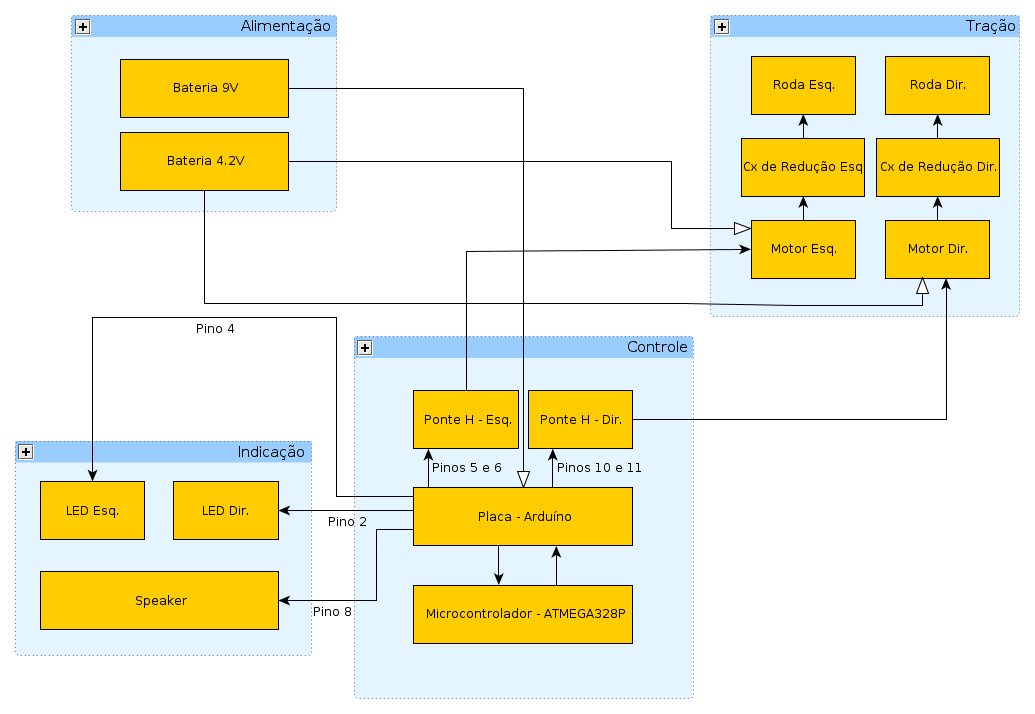
\includegraphics[scale=0.3]{imagens/robo.png}
    \caption{Diagrama do Robô}
    \label{int_fig01}
\end{figure}

\subsection{Sistema de Alimentação}

Conjunto de baterias utilizadas como alimentação do robô.

\subsubsection{Bateria de 9V}
Utilizada para alimentação do \textit{Arduíno Duemilanove}, uma bateria PP3.

\subsubsection{Bateria de 4,2V}
Usada na alimentação dos motores, bateria de câmera fotográfica digital.

\subsubsection{Bateria de 6V}
Usada na alimentação da CMUCam3, quatro pilhas AA em série.

\subsection{Sistema de Indicação}

LEDs e \textit{Speaker} usados para indicar as ações do robô.

\subsubsection{LEDs}
Usados para indicação dos estados do robô, detalhados na Tabela \ref{int_tbl01}

\begin{table}[h!]
    \centering
    \begin{tabular}{|c|c|c|} \hline
        \textbf{Estado} & \textbf{LED Esquerdo} & \textbf{LED Direito} \\ \hline
        Parado & Apagado & Apagado \\ \hline
        Andando para frente & Aceso & Apagado \\ \hline
        Virando para esquerda & Aceso & Apagado \\ \hline
        Virando para direita & Apagado & Aceso \\ \hline
    \end{tabular}
    \caption{Sistema de Indicação}
    \label{int_tbl01}
\end{table}

\subsubsection{Speaker}
Utilizado como indicador sonoro de estados específicos do sistema, como reconhecimento do objeto e início e fim da busca do mesmo.

\subsection{Sistema de Tração}

Para tração do robô foi construído um sistema baseado em um motor elétrico e duas rodas centrais.

\subsubsection{Motores}
Motor elétrico de corrente contínua \textit{Tamiya} de 3V com rotação de 12300 rpm, ou 205 voltas por segundo \cite{RoboExplorador}

\subsubsection{Caixas de redução}
Acopladas ao motor e às rodas reduzem a rotação do motor para que seja possível acionar as rodas. Na configuração usada, a redução é de 344:1 \cite{RoboExplorador}.

\subsubsection{Rodas}
O robô utiliza duas rodas \textit{off-road} em seu centro e uma esfera com giro livre atrás para manter o equilíbrio.

Com a rotação de 205 voltas/segundo e a redução de 344:1, a roda completa 0,6 voltas por segundo.

\subsection{Sistema de Controle}

Sistema para controle da movimentação do robô.

\subsubsection{Ponte H} 

A Ponte H é um circuito que permite a um microcontrolador acionar um motor de corrente contínua. Por questões eletrônicas \cite{RoboExplorador}, o circuito utilizado no projeto foi construído a partir de componentes discretos.

\subsubsection{Arduíno Duemilanove}

Placa \textit{Arduíno} utilizada no projeto anterior e reutilizada no projeto atual. Faz o interfaceamento dos diversos sistemas do projeto, \textit{i.e.}, recebe as decisões tomadas pelo Sistema de Navegação, embarcado na câmera, e aciona os motores para que o robô as execute. Seu funcionamento é detalhado na seção \ref{sec_arduino}.

\subsubsection{Microcontrolador ATMEGA328P}

Microcontolador presente da \textit{Arduíno Duemilanove}, os códigos construídos para controle do robô (Seção \ref{sec_soft_controle}) serão executados por ele.

\section{Plataforma Arduíno}
\label{sec_arduino}


\section{Software de Controle}
\label{sec_soft_controle}
